\documentclass[10pt,twocolumn,letterpaper]{article}

\usepackage{cvpr}
\input{preamble}
\definecolor{cvprblue}{rgb}{0.21,0.49,0.74}
\usepackage[pagebackref,breaklinks,colorlinks,allcolors=cvprblue]{hyperref}

\title{COMP4332 Project 1 Report}
\author{Group No.\ 21}
\def\paperID{}
\def\confName{COMP4332}
\def\confYear{2026 Spring}
\begin{document}

\maketitle

\section{Introduction}
\noindent This project studies a seven-class emotion classification on short texts, where each sample is assigned to one of the following labels: anger, disgust, fear, joy, neutral, sadness, or surprise. 
We use the dataset and the provided MLP and RNN baselines from the course skeleton, and extend the implementation by adding GRU and LSTM for comparison. 
Model performance is evaluated mainly with Macro-F1, which reflects performance across all classes rather than being dominated by the majority categories like joy. 
Among the four models, our GRU model achieves a validation Macro-F1 of 0.5668, which is noticeably better than the MLP and RNN baselines. 
We also experimented with different pretrained embedding models, which pushed the validation Macro-F1 above 0.60. 
This report summarizes our data processing pipeline, model selection and implementation, and the experimental results with corresponding analysis.

\section{Data Processing}

\subsection{Baseline pipeline}
\noindent As provided in the skeleton, we tokenise text on the training set, build a frequency-based vocabulary, map tokens to integer IDs, and pad or truncate sequences to a fixed length. An \texttt{nn.Embedding} layer converts these IDs into trainable vectors, which are fed into the trainable model head (we use several architectures, including those from the skeleton and our GRU/LSTM extensions) and updated end-to-end with the classification layer.

\subsection{Pretrained encoder embeddings}
\noindent We additionally use frozen token-level representations from large pretrained models such as CLIP and BERT. These encoders are trained on broad corpora and already encode latent and contextual regularities; we keep their parameters fixed and only train the downstream GRU/LSTM heads on top of their outputs.

\section{Model Selection and Implementation}

\paragraph{MLP and RNN.}
\noindent For the MLP and RNN baselines, we follow the course skeleton implementation: we use the provided tokenisation, vocabulary construction, embedding layers, model architectures, and training setup as distributed in the project starter code, and run them to obtain predictions for comparison with our extended models.

\paragraph{GRU and LSTM.}
\noindent Our GRU and LSTM models share the same setup on top of the skeleton data pipeline: a trainable embedding layer feeds a two-layer bidirectional recurrent encoder; we take the final forward and backward hidden states from the top layer, concatenate them into a single vector, and pass it through a linear classifier. We optimise with Adam and cross-entropy for 30 epochs and keep the checkpoint with the best validation Macro-F1 for prediction generation.
For the GRU variant, we replace the vanilla RNN cell with a bidirectional GRU, whose gating simplifies long-range credit assignment compared with a basic RNN.
The LSTM variant is obtained by the same recipe with only the recurrent core changed: we swap the GRU for an LSTM, which uses a separate memory cell and input/forget/output gates instead of GRU-style update and reset gates, while the stacking, bidirectionality, use of the top layer's last forward and backward hidden states, classifier head, and training protocol remain the same except for the LSTM learning rate in our implementation ($10^{-3}$ versus $5\times10^{-4}$ for GRU).

\section{Results and Analysis}

\noindent Figure~\ref{fig:f1-comparison} compares the per-class F1 scores and Macro-F1 of the four baseline models on the validation set, while Figure~\ref{fig:gru-confusion} further shows the confusion matrix of the GRU baseline.

\begin{figure*}[t]
\centering
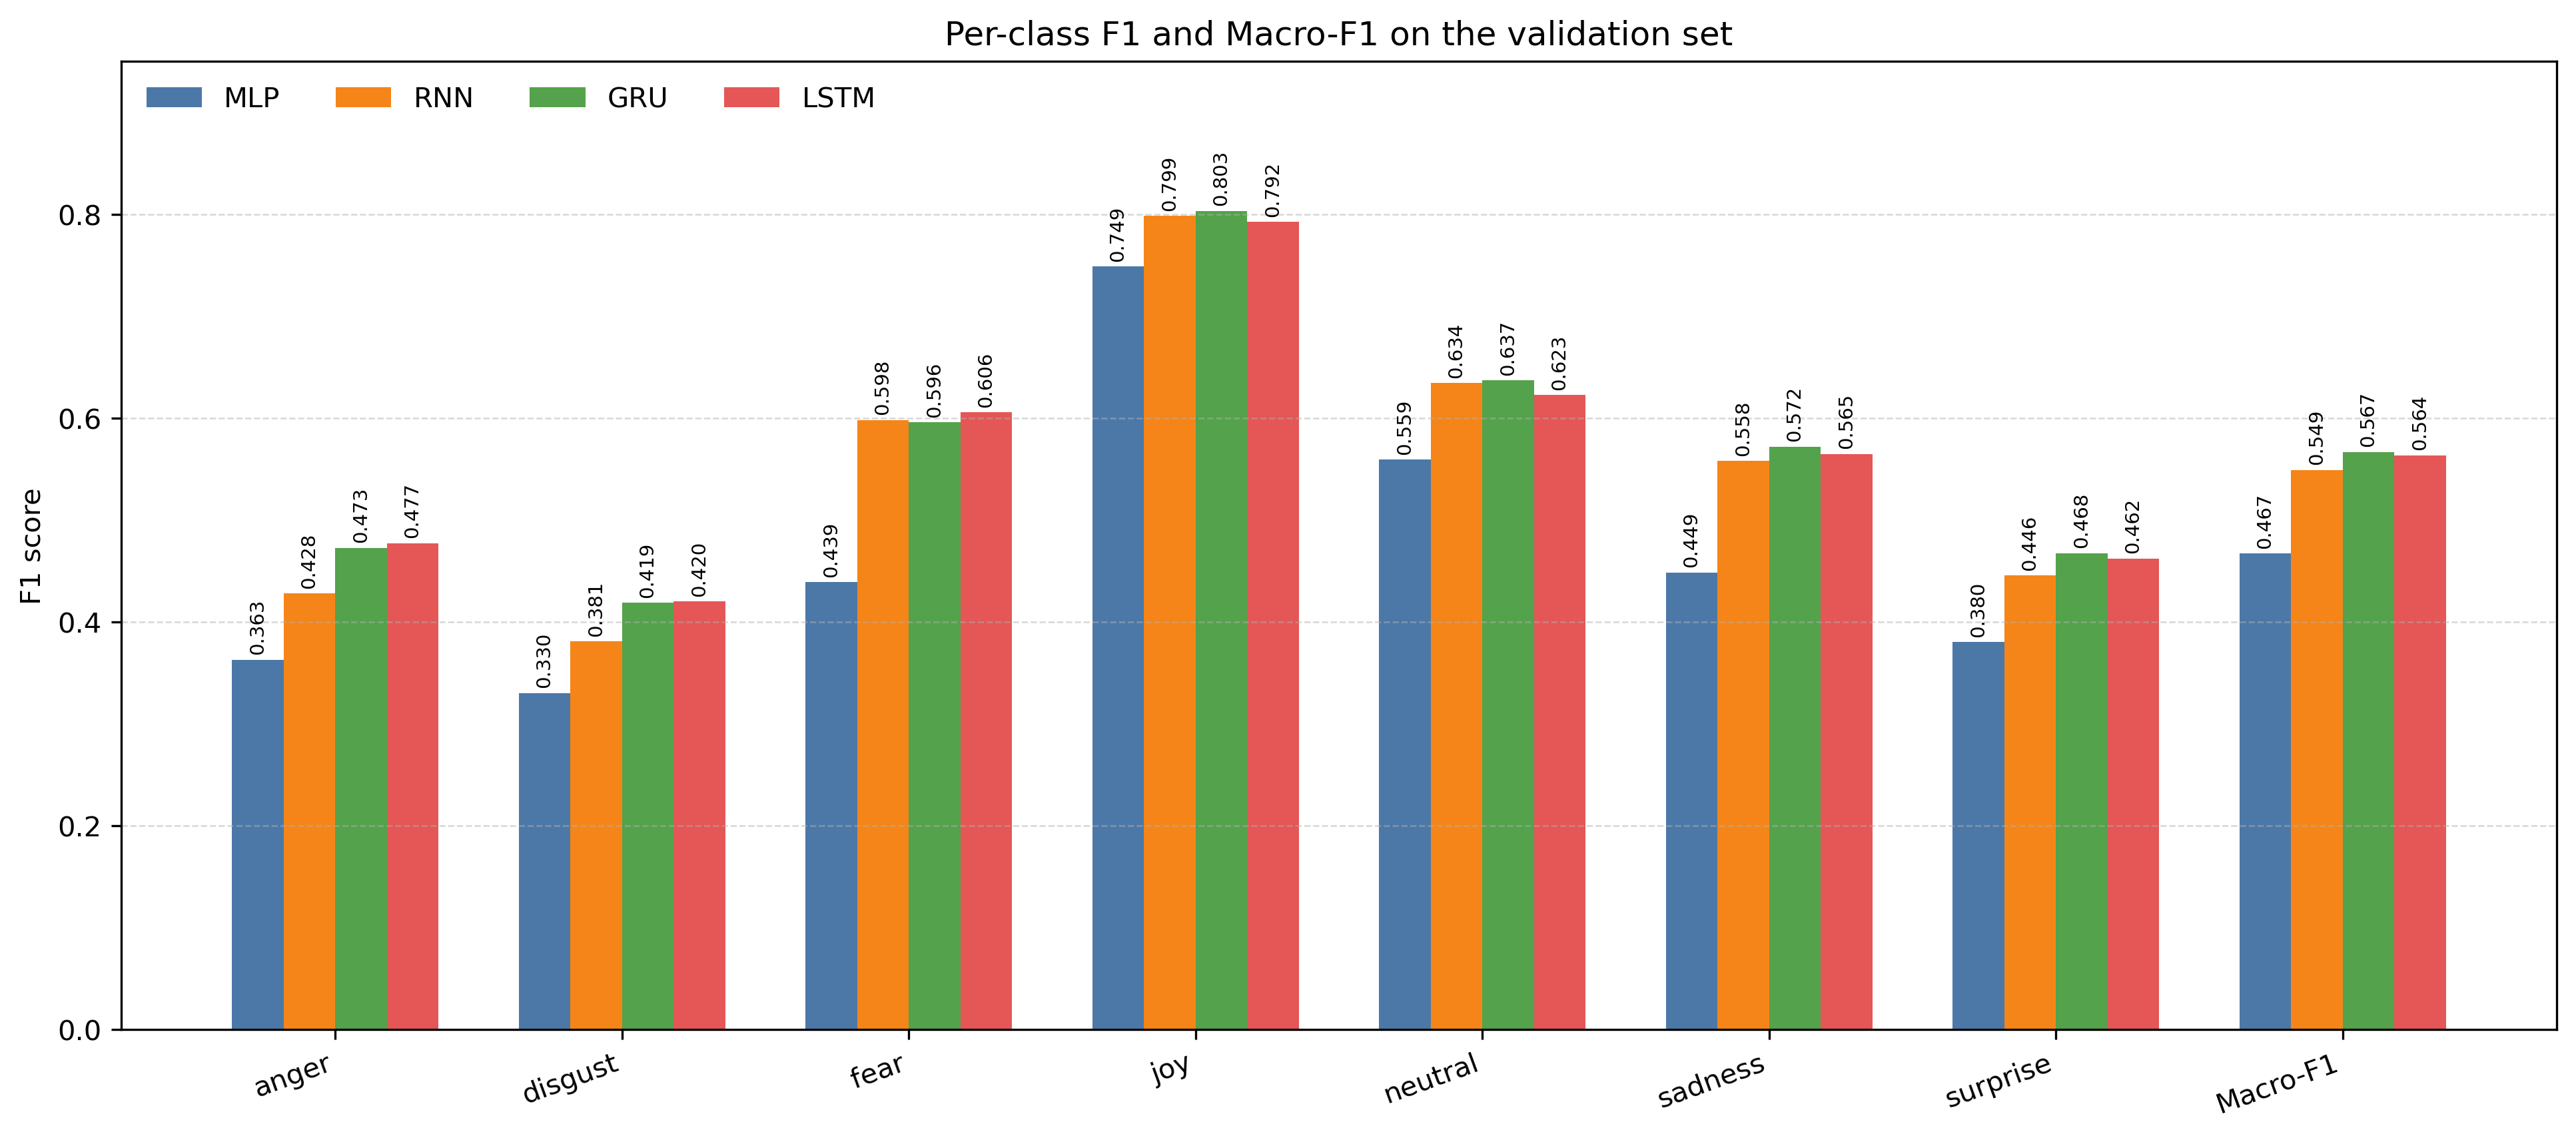
\includegraphics[width=\textwidth]{baseline_f1_comparison.png}
\caption{Per-class F1 scores and Macro-F1 of MLP, RNN, GRU, and LSTM on the validation set.}
\label{fig:f1-comparison}
\end{figure*}

\begin{figure}[t]
\centering
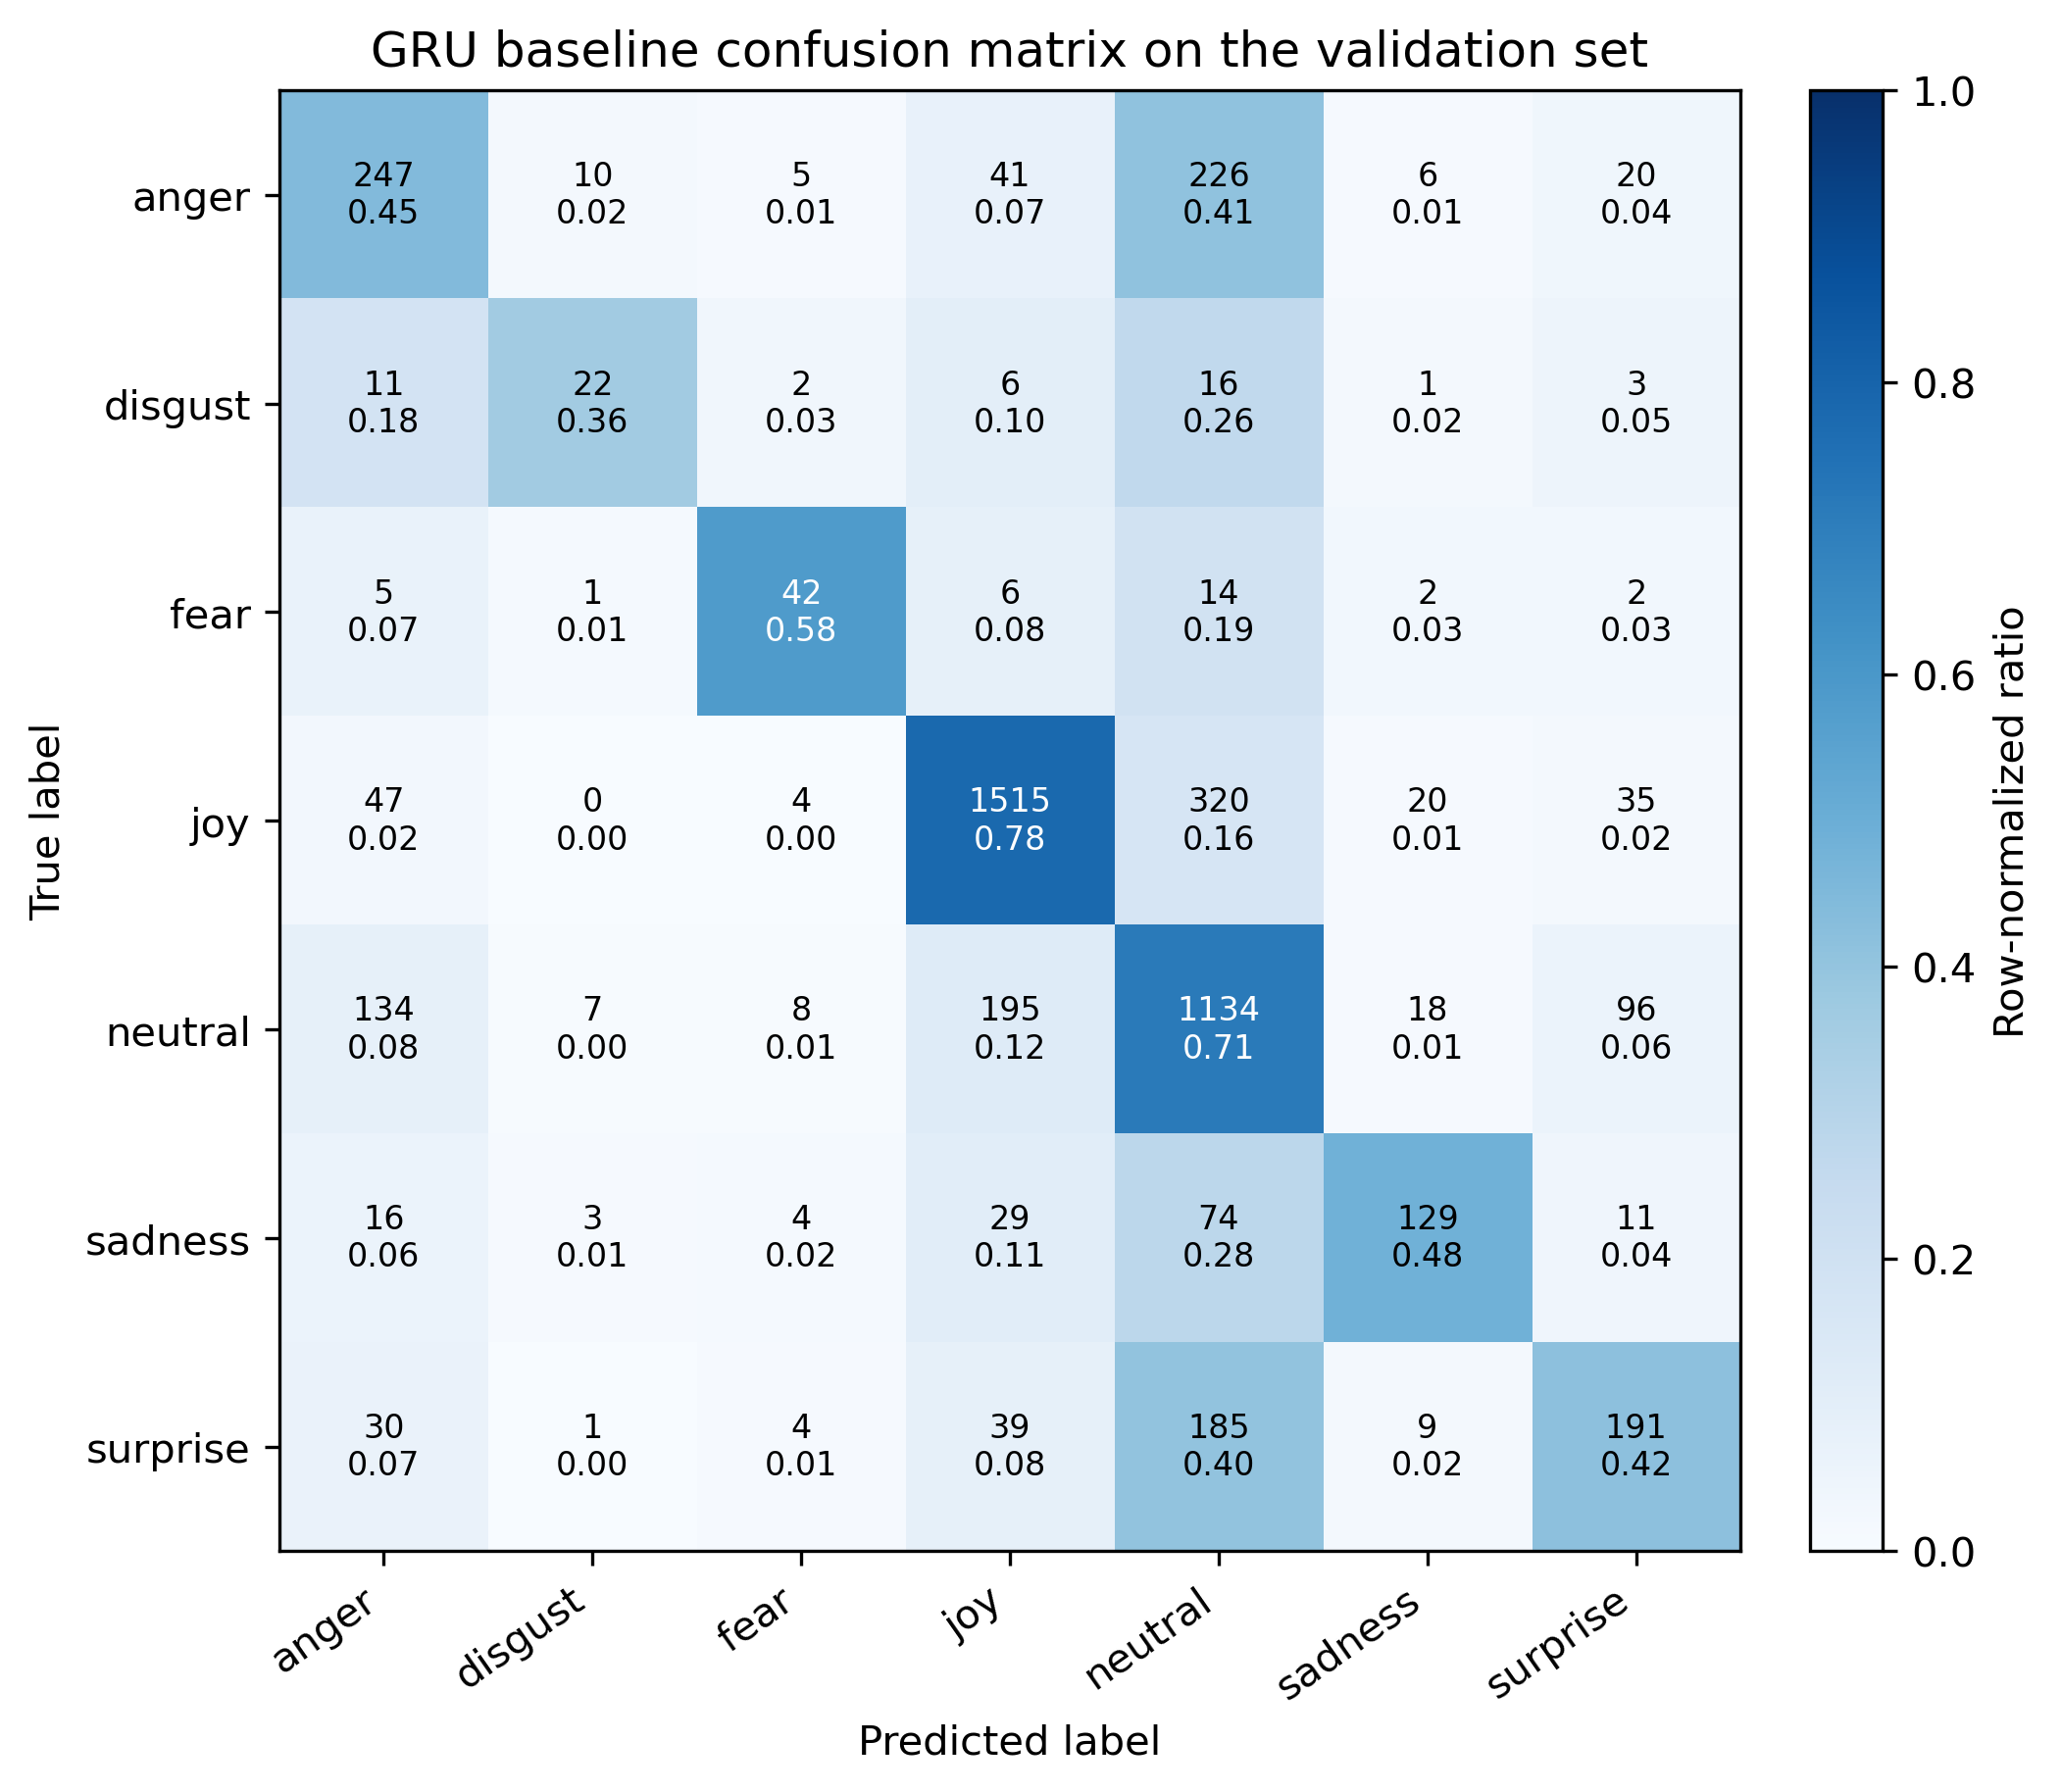
\includegraphics[width=\linewidth]{gru_confusion_matrix.png}
\caption{Confusion matrix of the GRU baseline on the validation set.}
\label{fig:gru-confusion}
\end{figure}

\noindent From Figure~\ref{fig:f1-comparison}, the overall ranking is clear: MLP gives the weakest Macro-F1 (0.467), RNN improves it to 0.549, and the two gated recurrent models perform best, with GRU slightly ahead of LSTM at 0.567 versus 0.564. This pattern suggests that modelling sequential context is necessary for emotion classification, and that gating helps the model preserve useful information better than a vanilla RNN.

\noindent Looking at the class-wise scores, joy is the easiest class for all models, with F1 close to 0.8 for the recurrent models, while disgust, anger, and surprise remain much harder. This imbalance is consistent with the nature of the dataset: joy and neutral appear more frequently and have more stable lexical patterns, whereas minority emotions are less represented and often overlap semantically with other affective categories.

\noindent Figure~\ref{fig:gru-confusion} helps explain why GRU performs best overall but still has limitations. The diagonal entries are strongest for joy (0.78) and neutral (0.71), confirming that the model recognises the dominant classes relatively well. However, there is substantial confusion between anger and neutral, surprise and neutral, and sadness and neutral. For example, 41\% of anger samples are predicted as neutral, and 40\% of surprise samples are also mapped to neutral. This shows that the model tends to fall back to broad or less emotionally marked categories when the input signal is ambiguous.

\noindent Overall, the two figures together show that GRU offers the best balance among the baseline models: it improves Macro-F1 across most classes, especially compared with MLP and vanilla RNN, but the remaining errors indicate that minority emotions and closely related labels are still challenging under the basic embedding pipeline.

\noindent Besides the baseline comparison, we also conduct supplementary experiments with frozen pretrained embeddings to test whether stronger input representations can further improve the recurrent models.

\begin{table}[t]
\centering
\begin{tabular}{lcc}
\hline
Model & Accuracy & Macro-F1 \\
\hline
CLIP + GRU  & 0.6884 & 0.6037 \\
CLIP + LSTM & 0.6773 & 0.5938 \\
BERT + GRU  & 0.6789 & 0.6049 \\
BERT + LSTM & 0.6909 & 0.5968 \\
\hline
\end{tabular}
\caption{Validation results of GRU and LSTM with frozen pretrained embeddings.}
\label{tab:pretrained-results}
\end{table}

\noindent Table~\ref{tab:pretrained-results} shows that pretrained embeddings consistently improve the recurrent models over the basic embedding pipeline. All four variants achieve Macro-F1 close to or above 0.59, which is higher than the baseline GRU and LSTM results. This indicates that CLIP and BERT provide richer semantic information than embeddings learned only from the training set, allowing the classifier to better separate emotionally similar classes.

\noindent Among the supplementary settings, BERT + GRU achieves the best Macro-F1 of 0.6049, while BERT + LSTM obtains the highest accuracy of 0.6909. The gap between accuracy and Macro-F1 also suggests that overall correctness is not identical to balanced class performance: a model can classify common categories well without necessarily handling minority emotions equally well. Therefore, Macro-F1 remains the more informative metric for this task.

\noindent Combining the baseline figures and the supplementary experiment table, we observe a consistent trend: stronger sequence modelling improves performance first, and stronger pretrained representations bring an additional gain on top of that. This supports our conclusion that emotion classification benefits from both contextual recurrent encoders and semantically informative input embeddings.

\section{Conclusion}
\noindent In this project, we compared four text classification models for seven-class emotion recognition and observed a consistent improvement from simple baselines to stronger recurrent architectures. Under the basic embedding pipeline, GRU and LSTM both outperformed MLP and vanilla RNN, which confirms the importance of modelling sequential structure and longer contextual dependencies in this task.

\noindent We further improved the system by introducing frozen pretrained embeddings from CLIP and BERT. These pretrained representations provided stronger semantic features than embeddings learned only from the task data, and further boosted the performance of both GRU and LSTM. Our best result was achieved by BERT + GRU, which reached a validation Macro-F1 of 0.6049. Overall, the experiments show that combining pretrained embeddings with gated recurrent models is an effective approach for emotion classification on short texts.

\end{document}
